\documentclass[12pt, a4paper, times, capchap, capsec, floatnumber=continuous, header=yes]{abnt}
\usepackage[utf8]{inputenc} % acentos em portugues
\usepackage{graphicx} % importar imagens
\usepackage{sty/abnt-UFSC}
\usepackage{longtable,color}
\usepackage{amsmath}
\usepackage{amstext}
\usepackage{amsfonts}
\usepackage{amssymb}
\usepackage{array}
\usepackage{hyphenat}
\usepackage{url}
\usepackage{caption}
\usepackage{float}
\usepackage{listings}
\usepackage{textcomp}

\lstset{language=C,
numbers=left,
stepnumber=1,
firstnumber=1,
numberstyle=\tiny,
extendedchars=true,
breaklines=true,
frame=tb,
basicstyle=\footnotesize,
stringstyle=\ttfamily,
showstringspaces=false
}
\renewcommand{\lstlistingname}{C\'{o}digo Fonte}
\renewcommand{\lstlistlistingname}{Lista de C\'{o}digos Fonte}

\def\Versao$#1 #2${#2}
\def\Data$#1 #2 #3${#2}

\autor{Vitor Arins Pinto}
\titulo{Redes Neurais Convolucionais de Profundidade para Reconhecimento de Textos em Imagens de CAPTCHA.}
\orientador[]{Orientadora: Luciana de Oliveira Rech }
\comentario{Trabalho de Conclusão de Curso submetido ao Programa de
  graduação da Universidade Federal de Santa Catarina para a obtenção
  do Grau de Bacharel em Sistemas de Informação.}
\instituicao{Universidade Federal de Santa Catarina \par
    Centro Tecnológico \par
    Departamento de Informática e Estatística}
\local{Florian\'{o}polis}
\data{\today}


\begin{document}

\capa
\folhaderosto

\chapter*{Agradecimentos}

Primeiramente gostaria de agradecer à minha amada namorada e melhor
amiga Letícia, que além de me mostrar o real significado do amor e
me apresentar a felicidade de uma maneira que eu não conhecia,
cooperou no desenvolvimento do trabalho desde o seu início, suportando
amorosamente a minha ausência, se sobrecarregando com trabalho
(inclusive o de revisar esse texto) permitindo que eu me dedicasse
integralmente ao desenvolvimento do mesmo.

Aos meus pais agradeço por todo o esforço e sacrifício que fizeram
para que eu pudesse chegar aqui, sem eles eu certamente não teria
oportunidade de realizar este trabalho nem de viver todas as
experiências maravilhosas que tive até hoje.

Ao meu irmão Marcel por tudo que me ensinou e todos os conselhos que
me deu até hoje.

Agradeço à Marilene Bittencourt que sempre me incentivou a ser melhor
e há muito tempo dá ensinamentos que me levam para um caminho de
sucesso.

Ao meu mentor Eduardo Bellani por me guiar nos primeiros momentos
profissionais de minha carreira e também por abrir meus olhos diante
de claras observações dessa imensidão que chamamos de vida.

Agradeço a Neoway e todos os seus funcionários pelas oportunidades que
me foram dadas e por fornecer dados indispensáveis no desenvolvimento
deste trabalho.

Por fim agradeço a todos os professores da UFSC que tive contato, em
especial a minha orientadora Prof.ª Luciana de Oliveira Rech, Dr.ª e aos
membros da banca Prof. Mário Antônio Ribeiro Dantas, Dr. e Prof.ª 
Jerusa Marchi, Dr.ª.
\begin{resumo}
        
Atualmente, muitas aplicações na Internet seguem a política de manter
alguns dados acessíveis ao público. Para isso é necessário desenvolver
um portal que seja robusto o suficiente para garantir que todas as
pessoas possam acessá-lo. Porém, as requisições feitas para recuperar
dados públicos nem sempre vêm de um ser humano. Empresas
especializadas em Big data possuem um grande interesse em fontes de
dados públicos para poder fazer análises e previsões a partir de dados
atuais. Com esse interesse, \textit{Web Crawlers} são
implementados. Eles são responsáveis por consultar fontes de dados
milhares de vezes ao dia, fazendo diversas requisições a um
\textit{website}. Tal \textit{website} pode não estar preparado para
um volume de consultas tão grande em um período tão curto de
tempo. Com o intuito de impedir que sejam feitas consultas por
programas de computador, as instituições que mantêm dados públicos
investem em ferramentas chamadas CAPTCHA (teste de Turing público
completamente automatizado, para diferenciação entre computadores e
humanos). Essas ferramentas geralmente se tratam de imagens contendo
um texto qualquer e o usuário deve digitar o que vê na imagem. O
objetivo do trabalho proposto é realizar o reconhecimento de texto em
imagens de CAPTCHA através da aplicação de redes neurais
convolucionais.

\end{resumo}

\begin{abstract}

Currently many applications on the Internet follow the policy of keeping
some data accessible to the public. In order to do this, it's
necessary to develop a portal that is robust enough to ensure that all
people can access this data. But the requests made to recover
public data may not always come from a human. Companies
specializing in Big data have a great interest in data from public
sources in order to make analysis and forecasts from current 
data. With this interest, Web Crawlers are implemented. They are
responsible for querying data sources thousands of times a day,
making several requests to a website. This website may not be
prepared for such a great volume of inquiries in a short period of
time. In order to prevent queries to be made by
computer programs, institutions that keep public data
invest in tools called CAPTCHA (Completely Automated Public
 Turing test to tell Computers and Humans Apart). These tools usually deal
with images containing text and the user must enter what he or she
sees in the image. The objective of the proposed work is to perform the
text recognition in CAPTCHA images through the application of
convolutional neural networks.

\end{abstract}


\listoffigures
\listoftables
% Para seguir um padrão, a lista de siglas fica em um arquivo
% separado e todas a suas configurações específicas são colocados
% neste arquivo.

\chapter*{Lista de abreviaturas e siglas}

\noindent
\verb"CAPTCHA" \dotfill \textit{Completely Automated Public Turing
  test to tell Computers and Humans Apart}\\
\verb"AWS" \dotfill \textit{Amazon Web Services}\\
\verb"IA" \dotfill \textit{Inteligência Artificial}\\
\verb"DCNN" \dotfill \textit{Deep Convolutional Neural Networks}\\
\verb"ReLU" \dotfill \textit{Rectified Linear Unit}\\
\verb"GPU" \dotfill \textit{Graphical Processing Unit}\\
\verb"GPGPU" \dotfill \textit{General Purpose Graphical Processing
  Unit}\\
\verb"MNIST" \dotfill \textit{Mixed National Institute of Standards
  and Technology}\\
\verb"RAM" \dotfill \textit{Random Access Memory}\\
\verb"ASCII" \dotfill \textit{American Standard Code for Information
  Interchange}\\
\verb"RGB" \dotfill \textit{Red Green Blue}\\

\sumario

\setcounter{page}{1}

\chapter{Introdução}

Redes neurais artificiais clássicas existem desde os anos 60, como fórmulas  
matemáticas e algorítimos. Atualmente os programas de aprendizado de máquina  
contam com diferentes tipos de redes neurais. Um tipo de rede neural muito  
utilizado para processamento de imagens é a rede neural convolucional de  
profundidade. O trabalho em questão tratará da utilização e
configuração de uma rede neural convolucional de profundidade para
reconhecimento de textos em imagens específicas de CAPTCHAs.

\section{Problema}

Com o aumento constante na quantidade de informações geradas e 
computadas atualmente, percebe-se o surgimento de uma necessidade de tornar
alguns tipos de dados acessíveis a um público maior. A fim de gerar
conhecimento, muitas instituições desenvolvem portais de acesso para
consulta de dados relevantes a cada pessoa. Esses portais, em forma de
aplicações na Internet, precisam estar preparados para receber
diversas requisições e em diferentes volumes ao longo do tempo.

Devido a popularização de ferramentas e aplicações especializadas em Big
data, empresas de tecnologia demonstram interesse em recuperar grandes
volumes de dados de diferentes fontes públicas. Para a captura de tais
dados, \textit{Web crawlers} são geralmente implementados para a
realização de várias consultas em aplicações que disponibilizam dados
públicos.

Para tentar manter a integridade da aplicação, as organizações que possuem  
estas informações requisitadas investem em ferramentas chamadas CAPTCHA  
(teste de Turing público completamente automatizado para diferenciação entre  
computadores e humanos). Essas ferramentas frequentemente se tratam de  
imagens contendo um texto qualquer e o usuário precisa digitar o que vê na  
imagem. 

O trabalho de conclusão de curso proposto tem a intenção de retratar a  
ineficiência de algumas ferramentas de CAPTCHA, mostrando como redes neurais  
convolucionais podem ser aplicadas em imagens a fim de reconhecer o texto  
contido nestas imagens. 

\section{Objetivos}

\subsection{Objetivo geral}

Analisar o treinamento e aplicação de redes neurais convolucionais de
profundidade para o reconhecimento de texto em imagens de CAPTCHA.

\subsection{Objetivos específicos}

\begin{itemize}
        \item Estudar trabalhos correlatos e analisar o estado da arte;
	\item Entender como funciona cada aspecto na configuração de
          uma rede neural convolucional;
	\item Realizar o treinamento e aplicação de uma rede neural
          artificial para reconhecimento de CAPTCHAs.
\end{itemize}

\section{Escopo do trabalho}

O escopo deste trabalho inclui o estudo e análise de uma rede neural
convolucional de profundidade para reconhecimento de texto em imagens de 
um CAPTCHA específico.

Não está no escopo do trabalho:

\begin{itemize}
  \item Analisar outras formas de inteligência no reconhecimento de
    texto. 
  \item O estudo, análise ou implementação da aplicação de redes
    neurais convolucionais para outros tipos de problemas. 
  \item O estudo, análise ou implementação de softwares do tipo
    ``crawler'' ou qualquer programa automatizado para recuperar
    quaisquer informações de websites públicos.
  \item A análise e comparação de diferentes técnicas ou parâmetros
    para otimização de redes neurais.
\end{itemize}

\section{Metodologia}

Para realizar o proposto, foram feitas pesquisas em base de dados tais
como IEE Xplorer e ACM Portal. Adquirindo assim maior conhecimento
sobre o tema, estudando trabalhos relacionados. 

Com base no estudo do estado da arte, foram feitas pesquisas e
estudos para indicar caminhos possíveis para desenvolvimento da
proposta de trabalho.

\section{Estrutura do trabalho}

Para uma melhor compreensão e separação dos conteúdos, este trabalho
está organizado em 6 capítulos. Sendo este o capítulo 1 cobrindo a
introdução ao tema, citando os objetivos e explicando a proposta.

O capítulo 2 apresenta a fundamentação teórica, com as definições das
abordagens de desenvolvimento de aprendizado de máquina e redes
neurais. Também são apresentados alguns conceitos de tipos de redes
neurais.

No capítulo 3 está a proposta de experimento a ser realizado. Assim
como uma breve ideia dos resultados esperados e a forma de avaliação
dos mesmos.

O capítulo 4 contém as informações do desenvolvimento do treinamento
da rede neural para reconhecimento de imagens de CAPTCHA.

No capítulo 5 são apresentados os testes do treinamento da rede neural
para reconhecimento de imagens de CAPTCHA. Também a apresentação dos
dados obtidos através das metodologias escolhidas no capítulo 4.

Por fim, no capítulo 6 estão as conclusões obtidas através dos
resultados deste trabalho, as vulnerabilidades que podem comprometer o
acesso à dados públicos disponbilizados e as sugestões para trabalhos
futuros relacionados.
\chapter{Fundamentação Teórica}

\section{Aprendizado de máquina}

Aprendizado de máquina, ou \textit{Machine Learning}, é uma área da
computação que emergiu de estudos relacionados ao reconhecimento de
padrões e inteligência artificial. Nesta área é contemplado o estudo e
implementação de algoritmos que conseguem aprender e fazer previsões
baseadas em dados. Esses algoritmos funcionam através da construção de
um modelo preditivo que tem como entrada um conjunto de treinamento
com dados de observações quaisquer. Desse modo as previsões são feitas
orientadas aos dados e não a partir de instruções estáticas de um
programa.

\section{Redes Neurais}

Diante das ferramentas disponíveis que tratam de aprendizado de
máquina, uma delas é a rede neural artificial.

Redes neurais artificiais são conjuntos de modelos inspirados por
redes neurais biológicas, usados para aproximar funções que dependem
de um número muito grande de entradas. De acordo com Mackay\cite{Mackay},
Redes neurais geralmente são especificadas utilizando 3 coisas:

\begin{itemize}

\item {\bf Arquitetura:} Especifica quais variáveis estão envolvidas
  na rede e quais as relações topológicas. Por exemplo, as variáveis
  envolvidas em uma rede neural podem ser os pesos das conexões entre
  os neurônios.

\item {\bf Regra de atividade:} A maioria dos modelos de rede neural
  tem uma dinâmica de atividade com escala de tempo curta. São regras
  locais que definem como as \textit{atividades} de neurônios mudam em
  resposta aos outros. Geralmente a regra de atividade depende dos
  parâmetros da rede.

\item {\bf Regra de aprendizado:} Especifica o modo com que os pesos
  da rede neural muda conforme o tempo. O aprendizado normalmente toma
  uma escala de tempo maior do que a escala referente a dinâmica de
  atividade. Normalmente a regra de aprendizado dependerá das
  \textit{atividades} dos neurônios. Também pode depender dos valores
  que são objetivos definidos pelo usuário e valores iniciais dos
  pesos.

\end{itemize}

Tomando imagens como exemplo, uma rede neural para reconhecimento de
texto pode ter como entrada o conjunto de pixels da imagem. Depois de
serem atribuídos os pesos para cada item da entrada, os próximos
neurônios serão ativados mediante a função de atividade
pré-definida. Os pesos são recalculados através da regra de
aprendizado e todo processo é repetido até uma condição determinada
pelo usuário.

\section{Convoluções}

Para entender redes neurais convolucionais, é necessário primeiro
entender o que são convoluções. Segundo Olah\cite{Olah}, uma
convolução pode ser vista como um somatório das probabilidades de
resposta de duas funções algébricas. Tendo como definição padrão de
convolução a seguinte expressão:

\begin{equation}
   (f*g)(c) = \sum\limits_{a}f(a)\cdot g(c-a)
\end{equation}

Onde {\bf \emph{f}} e {\bf \emph{g}} são duas funções, {\bf \emph{c}}
é o parâmetro de entrada para a função final e {\bf \emph{a}} é um
parâmetro de entrada escolhido para uma das funções, geralmente uma
diferença temporal.

Como podemos considerar que imagens são funções bidimensionais, é
comum realizar transformações por meio de convoluções. Estas
convoluções são executadas com uma função local pequena chamada de
``kernel''.

\begin{figure}[H]
\centering
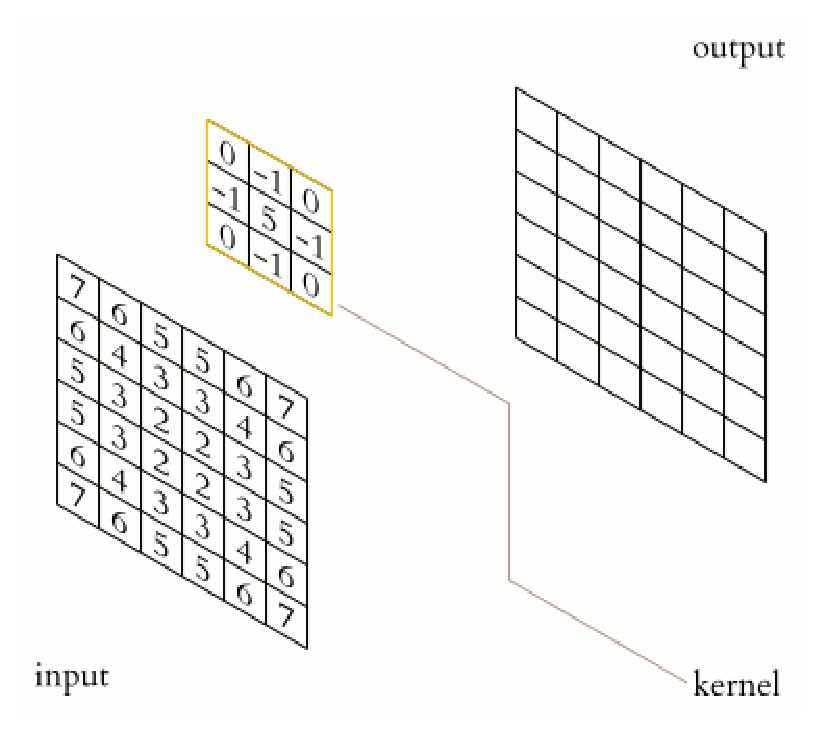
\includegraphics[scale=0.6]{imagens/fig1.eps}
\caption{Aplicação de uma função ``kernel'' sobre a função de uma
  imagem que é o ``input''.}
\label{fig:convolution_kernel}
\end{figure}

\subsection{Aplicação em redes neurais}

Redes neurais convolucionais são muito similares a redes neurais
comuns. De acordo com Karpathy\cite{Karpathy}:
\begin{quote}
  ``Arquiteturas de redes convolucionais assumem explicitamente que as
  entradas são imagens, o que nos permite cifrar algumas propriedades
  dentro da arquitetura. Essas então fazem a função de ativação mais
  eficiente de implementar e reduz drasticamente a quantidade de
  parâmetros na rede.'' (KARPATHY, 2015, tradução nossa).
\end{quote}

Portanto para o caso de reconhecimento de texto em imagens, as redes
neurais convolucionais fazem muito sentido.

\section{Aprendizado em profundidade}

O aprendizado em profundidade permite que modelos computacionais
compostos por múltiplas camadas de processamento possam aprender
representações de dados com múltiplos níveis de abstração\cite{LeCun}.

A solução de \textit{Deep learning} permite que computadores aprendam
a partir de experiencias e entendam o mundo em termos de uma
hierarquia de conceitos, com cada conceito definido em termos da sua
relação com conceitos mais simples. Juntando conhecimento de
experiência, essa abordagem evita a necessidade de ter operadores
humanos especificando formalmente todo o conhecimento que o computador
precisa. A hierarquia de conceitos permite que o computador aprenda
conceitos complexos construindo-os à partir de conceitos mais
simples. Desenhando um gráfico que mostra como esses conceitos são
construídos em cima de outros, o gráfico fica profundo, com muitas
camadas. Por esta razão, essa abordagem para IA é chamada de
Aprendizado em profundidade\cite{Goodfellow-et-al-2016-Book}.

\section{Redes neurais convolucionais de profundidade}

Ao combinar o aprendizado em profundidade com redes convolucionais,
conseguimos tratar problemas muito mais complexos de classificação em
imagens. Assim problemas mais simples, como o reconhecimento de
textos, podem ser resolvidos cada vez mais rápido e facilmente.

A grande vantagem na abordagem de redes neurais convolucionais de
profundidade (DCNN) para reconhecimento é que não é necessário um
extrator de características desenvolvido por um ser humano. Nas
soluções de \cite{Krizhevsky} e \cite{Goodfellow} é possível perceber
que foram usadas diversas camadas para o aprendizado das
características.

Em arquiteturas de profundidade, as funções de ativação dos neurônios
são unidades lineares retificadas (ReLU). Isso simplifica o uso de
\textit{backpropagation} e evita problemas de saturação, fazendo o
aprendizado ficar muito mais rápido.

\begin{figure}[H]
\centering
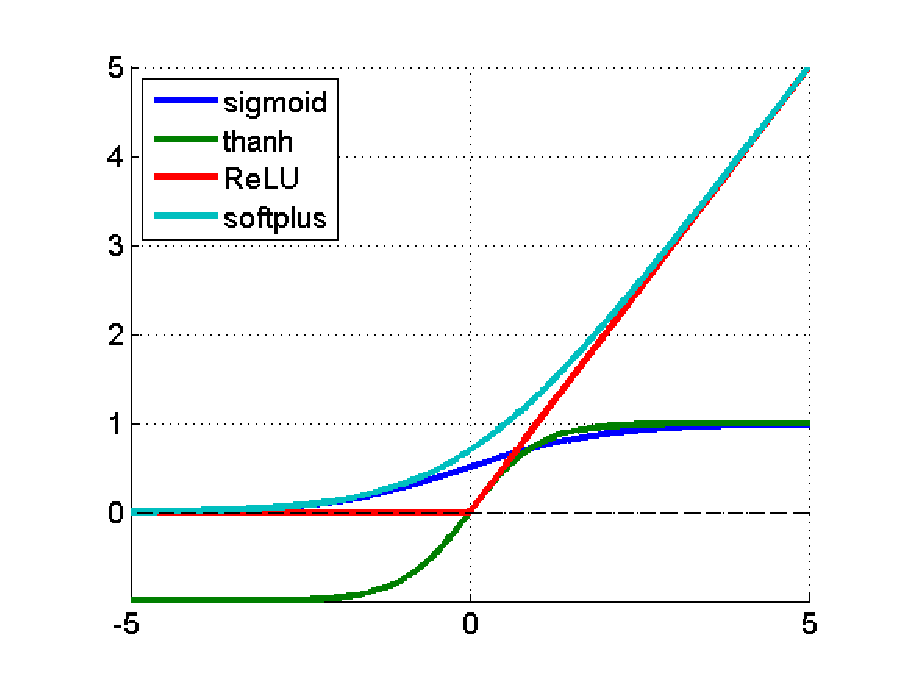
\includegraphics[scale=0.6]{imagens/activation_funcs.eps}
\caption{Comparação de funções de ativação.}
\label{fig:activation_funcs}
\end{figure}

DCNNs são a primeira abordagem verdadeiramente bem sucedida em
aprendizado em profundidade onde muitas camadas de uma hierarquia são
treinadas com sucesso de uma maneira robusta. Uma DCNN é uma escolha
de topologia ou arquitetura que se aproveita de relações espaciais
para reduzir o número de parâmetros que devem ser aprendidos, e assim
melhora o treinamento diante de uma rede com \textit{feed-forward
  backpropagation}\cite{Arel2010}.

\chapter{Proposta de experimento} \label{proposta}

Para realizar o experimento será necessário treinar um modelo de rede
neural que seja capaz, ou esteja próximo, de decifrar um CAPTCHA. Para
isso serão efetuadas três etapas básicas e comuns quando se trabalha
com redes neurais. Primeiro será coletado o maior número possível de
imagens de CAPTCHA. Em seguida será gerado um \textit{dataset} com as
características dessas imagens junto com a classe em que pertence. A
partir daí é possível realizar a configuração e treinamento da rede
neural. E por fim será calculada a acurácia, mediante imagens de
teste, do modelo que teve a melhor performance no treinamento.

\section{Coleta de imagens}

Como o escopo do trabalho não contempla a automatização da recuperação
de informações de \textit{websites} públicos, foi disponibilizado um
repositório com as imagens necessárias. Esse repositório possui
206.564 imagens e foi disponibilizado pela empresa Neoway. As imagens
se tratam de um CAPTCHA publicado pelo site do SINTEGRA de Santa
catarina
(\url{http://sistemas3.sef.sc.gov.br/sintegra/consulta_empresa_pesquisa.aspx}).

\begin{figure}[H]
\centering

\includegraphics[scale=1]{imagens/exemplo_captcha}
\caption{Um exemplo do CAPTCHA utilizado pelo sistema de consulta do
  SINTEGRA de Santa Catarina.}
\label{fig:exemplo_captcha}
\end{figure}


\subsection{Fonte pública}

Para demonstrar a ineficiência de certas imagens de CAPTCHA foi
escolhido um software Web. Este software do SINTEGRA, fornece dados
públicos de contribuintes mediante consulta via website. O SINTEGRA é
o Sistema Integrado de Informações sobre Operações Interestaduais com
Mercadorias e Serviços. Esta fonte pública possui dados fornecidos
pelos próprios contribuintes na hora do cadastro. Os comerciantes ou
profissionais autônomos fazem seu cadastro para facilitar o comércio
de produtos e prestação de serviços. O cadastro contempla inscrição da
pessoa física ou jurídica, endereço e informações complementares
referentes ao fisco estadual.

\section{Geração do Conjunto de dados}

O conjunto de dados (ou \textit{``dataset''}) que alimenta a rede neural é
gerado em tempo de execução do treinamento. Cada imagem é lida de seu
diretório em disco e carregada na memória como uma matriz de valores
de pixel. Ao final deste processo há um vetor em memória com todas
imagens existentes já pré-processadas. Isso é feito para o \textit{dataset} de
treinamento e de teste. O \textit{dataset} de treinamento terá a maioria das
imagens, que significa {\bf 180 mil} imagens para o contexto do
trabalho.

\subsection{Pré-processamento}

A fase de pré-processamento das imagens é mínima e é feita junto com a
geração do conjunto de dados.

\begin{itemize}
\item{\bf Escala de cinza}

Ao gerar um \textit{array} representativo da imagem, apenas é
considerado um valor de escala de cinza da imagem, assim padronizando
os valores de intensidade de pixels entre 0 e 1.

\item{\bf Redimensionamento}

Ao gerar o \textit{array} que representa a imagem, é feito um cálculo
para diminuir a imagem com base em uma escala. Essa escala será
configurada à partir de um valor padrão para a largura e altura das
imagens. 

\end{itemize}

\subsection{Conjunto de dados de teste}

Para o treinamento será necessário um conjunto separado para teste que
não possui nenhuma imagem presente no conjunto de treinamento.
O \textit{dataset} de testes terá uma amostra bem menor que o conjunto de
treinamento, portanto terá {\bf 8 mil} imagens.

\section{Treinamento}

Após gerado o conjunto de dados, é possível trabalhar no treinamento
do modelo da rede neural. Para isso será usado o \textit{framework}
{\bf \emph{TensorFlow}}\cite{TensorFlow} destinado à \textit{Deep
  Learning}. Também será desenvolvido um \textit{script} em
\textit{Python} que fará uso das funções disponibilizadas pela
biblioteca do \textit{TensorFlow}. Assim realizando o treinamento até
atingir um valor aceitável de acerto no conjunto de teste. O resultado
do treinamento será um arquivo binário representando o modelo que será
utilizado para avaliação posteriormente.

\subsection{Infraestrutura}

Com o intuito de acelerar o processo, foi utilizada uma
máquina com {\bf GPU} para o treinamento. A máquina foi adquirida em
uma \textit{Cloud} privada virtual da AWS\cite{GPUinstance}. A GPU
utilizada se trata de uma \textit{NVIDIA K80} com 2.496 cores e 12GB
de memória de vídeo. Como processador a máquina possui um
\textit{Intel Xeon E5-2686v4 (Broadwell)} com 4 cores, e ainda
possui 61GB de memória RAM.

\subsection{Bibliotecas utilizadas}

Todo o código foi implementado utilizando a linguagem de programação
{\bf \emph{Python}}, e as seguintes bibliotecas foram utilizadas:

\begin{itemize}

\item {\bf TensorFlow}\cite{TensorFlow}: Um \textit{framework}
  implementado em \textit{Python} destinado à \textit{Deep
    Learning}. Proporciona a criação da arquitetura e automatização do
  processo de treinamento de redes neurais com
  \textit{backpropagation}.

\item {\bf NumPy}\cite{NumPy}: Uma biblioteca em \textit{Python}
  criada para computação científica. Possui um objeto de
  \textit{array} com várias dimensões e várias funções sofisticadas
  para cálculos com algebra linear.

\item {\bf OpenCV}\cite{OpenCV}: Uma biblioteca, implementada em
  C/C++, destinada à computação visual. Utilizada para ler imagens em
  disco e realizar o pré-processamento nas mesmas.

\end{itemize}

\section{Avaliação de acurácia}

Para a avaliação, uma nova amostra de imagens será coletada do mesmo
modo que foram coletadas as imagens para treinamento. Essa amostra
terá uma quantidade maior de imagens do que o conjunto de teste.

Com essa amostra de imagens, será feita a execução do teste do modelo
contra cada uma das imagens, assim armazenando uma informação de erro
ou acerto do modelo. Ao final da execução será contabilizado o número
de acertos e comparado com o número total da amostra de imagens para
avaliação. Resultando assim em uma porcentagem que representa a
acurácia do modelo gerado.



\bibliography{ref}

\end{document}
